
\documentclass[11pt]{article}   	% use "amsart" instead of "article" for AMSLaTeX format
\usepackage{geometry}                		% See geometry.pdf to learn the layout options. There are lots.
\usepackage{tikz}
\geometry{letterpaper}                   		% ... or a4paper or a5paper or ... 
%\geometry{landscape}                		% Activate for for rotated page geometry
%\usepackage[parfill]{parskip}    		% Activate to begin paragraphs with an empty line rather than an indent
\usepackage{graphicx}				% Use pdf, png, jpg, or eps§ with pdflatex; use eps in DVI mode
\usepackage{amssymb}
\usepackage[document]{ragged2e}
\usepackage{array}
\usepackage{tabu}
\usepackage{pgf}
\usepackage{tikz}
\usetikzlibrary{positioning}
\usepackage{tikz,fullpage}
\usetikzlibrary{arrows,%
                petri,%
                topaths}%
\usepackage{tkz-berge}
\usepackage[position=top]{subfig}
\usepackage{enumitem}
\usepackage[utf8]{inputenc}
\usepackage[english]{babel}
 \usepackage{hyperref}


\title{Bioinformatics HAL application}
\author{James Duin}
\date{2-17-2016}							% Activate to display a given date or no date

\begin{document}
\maketitle


\begin{enumerate}[ label=\textbf{\Roman*.},listparindent=1.5em] % start the problems

\item Simulate the system and show plots: \\
	\par The following plots were obtained with a round batch size of 100
	and a starter set of 1040 instances out of the total 2098 instances.
	The plots are the average of 10 folds, for each fold a test set of 2010
	containing representatives of each class was held out, out of the remaining
	18088, the starter set was selected which again contained representatives of
	each class. Coarse and fine classifiers share the same starter set. During
	 each round coarse and fine classifiers are trained on their corresponding
	 sets, metrics are outputted on the held out test set, then confidence estimates
	 are ran on the remaining eligible instances. Eligible instances are kept in
	 separate sets for coarse and fine, 100 of the most uncertain instances are removed
	 from each eligible set and added to its corresponding coarse or fine set to be
	 trained on for the next round.\\

\item Plots for Logistic Regression Active vs Passive curves: \\% start sect1
\begin{center}	
\makebox[\textwidth]{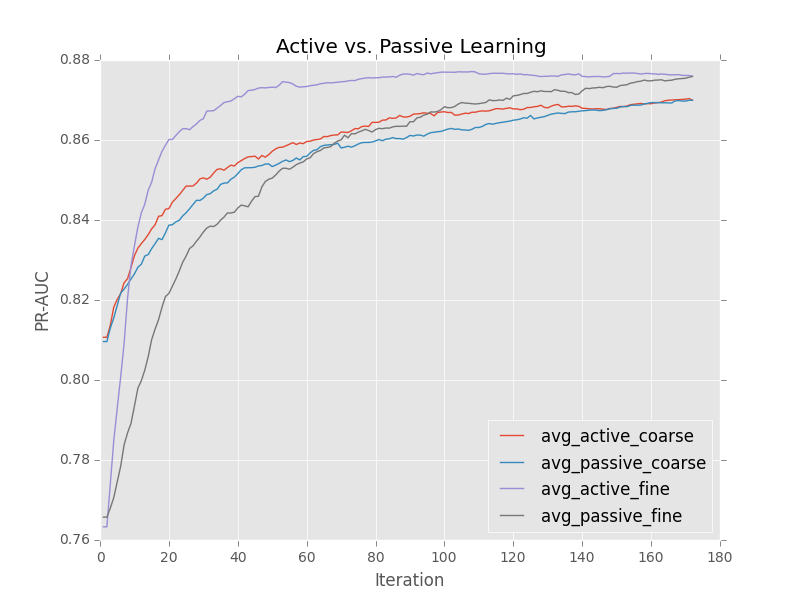
\includegraphics[ width=\paperwidth]{ActiveVsPassivePRLR}}
\par \textit{Figure:1}  The PR AUC curves for rounds with the Logistic
Regression classifier conforms to expectations, with active-fine having
the highest performance. Active-coarse outperforms passive-coarse. Passive-fine
doesn't outperform the coarse classifiers until rnd 100. \\
\makebox[\textwidth]{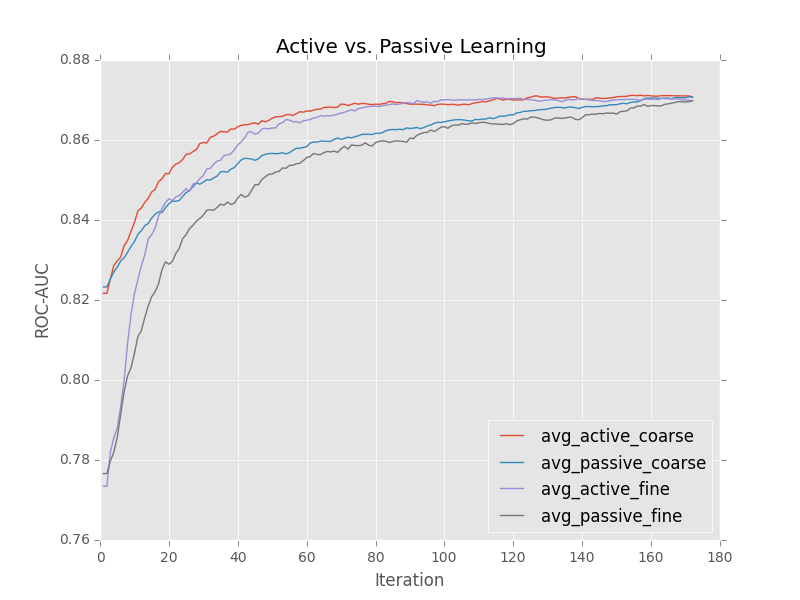
\includegraphics[width=\paperwidth]{ActiveVsPassiveROCLR}}
\par \textit{Figure:2}  The ROC AUC curves for rounds with the
Logistic Regression classifier. The active curves beat out the passive
curves for both coarse and fine. Coarse roc starts with an advantage over
fine as in the PR curves. Both converge to the same rate after roc auc level after 80.\\
\makebox[\textwidth]{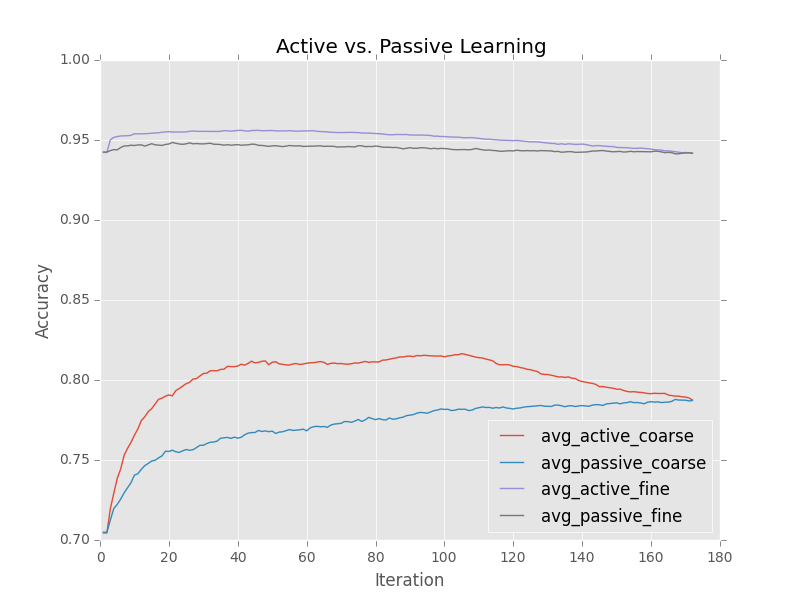
\includegraphics[width=\paperwidth]{ActiveVsPassiveAccLR}}
\par \textit{Figure:3}  The accuracy of the fine classifiers stays at
roughly the same rate throughout the rounds, this is due to an effective
weighting scheme for the fine grained classifiers. The active coarse accuracy
drops towards the end due to an increase in false positives as more negative
instances are added in the later rounds.\\
\makebox[\textwidth]{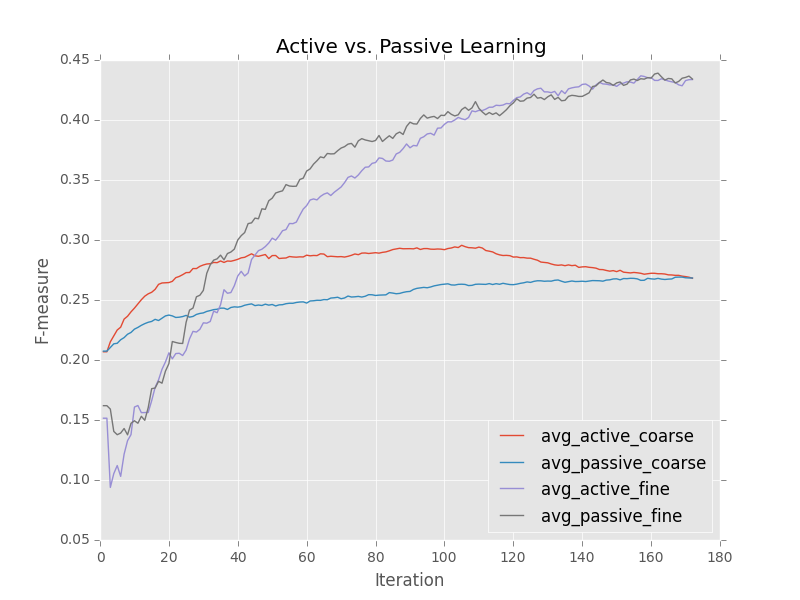
\includegraphics[width=\paperwidth]{ActiveVsPassiveF1LR}}
\par \textit{Figure:4}  The F-measure of the the fine classifiers increases
throughout the rounds as more true positives are predicted. The active coarse
again decreases at later rounds due to increased false positives.\\
\end{center}
\break





\item Plots for SVM Active vs Passive curves: \\% start sect1
\begin{center}	
\makebox[\textwidth]{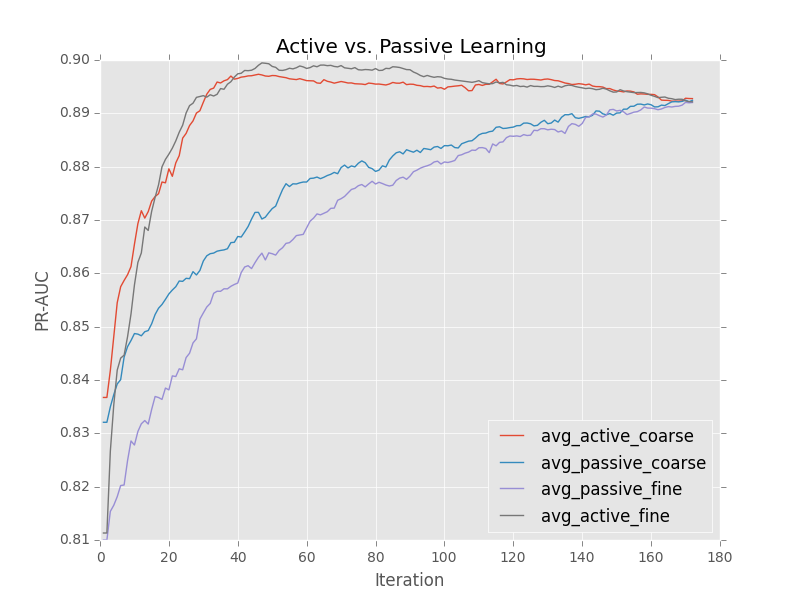
\includegraphics[ width=\paperwidth]{ActiveVsPassivePRSVM}}
\par \textit{Figure:3}   The PR AUC curves for rounds with SVM show little
advantage for fine. The results are slightly different than the ones shown
on 2/14 due to fixing a bug with the code that wasn't performing the
preprocessing scaling for the SVM case at the same stage as it was being
done for the logistic regression classifier.\\
\makebox[\textwidth]{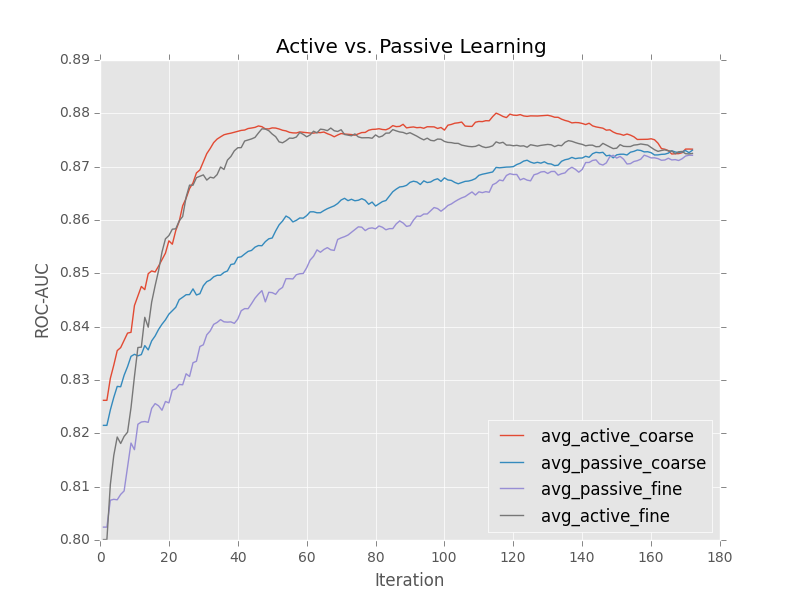
\includegraphics[width=\paperwidth]{ActiveVsPassiveROCSVM}}
\par \textit{Figure:4} The ROC curves show more of an advantage for coarse classifiers. \\
\makebox[\textwidth]{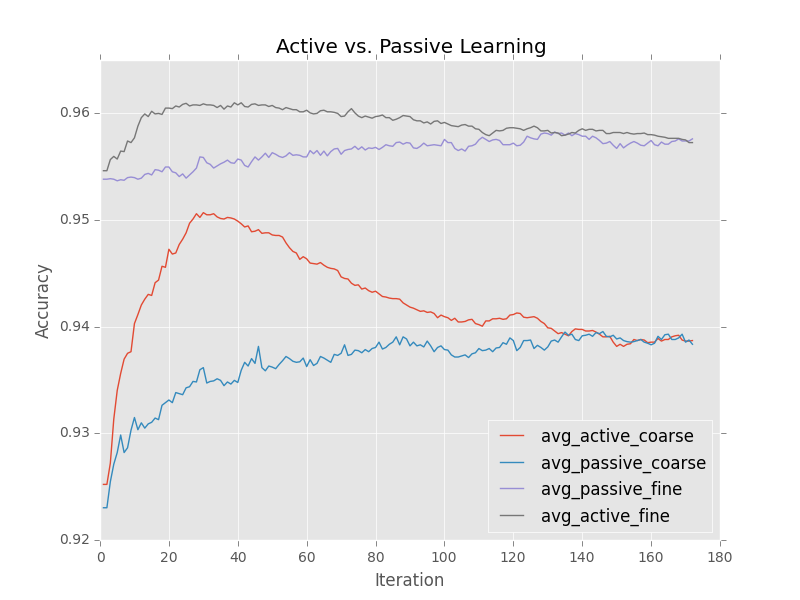
\includegraphics[width=\paperwidth]{ActiveVsPassiveAccSVM}}
\par \textit{Figure:5}  The accuracy for the coarse decreases sharply due
to coarse predicting steadily more false positives, behaving similar to the
Log Reg case. Fine accuracy is higher due to predicting less false positives
than coarse. Fine also predicts less true positives, compare apx. 37 to apx.
60 t.p. for coarse at round 60. \\
\makebox[\textwidth]{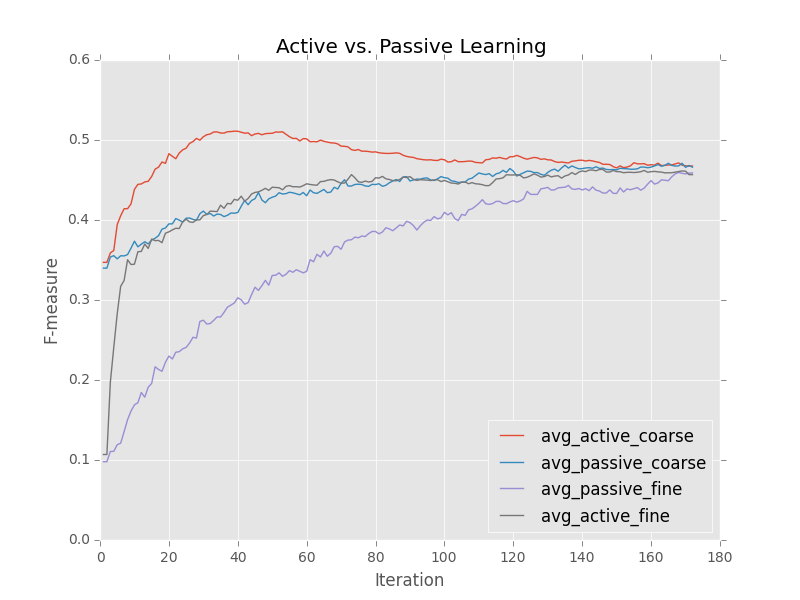
\includegraphics[width=\paperwidth]{ActiveVsPassiveF1SVM}}
\par \textit{Figure:6}  The F-measure favors coarse, and trends to the same level for both coarse and fine.\\
\end{center}

\break


\item Preliminary Plots for FFR experiments:\\% start sect1
\begin{center}	
\makebox[\textwidth]{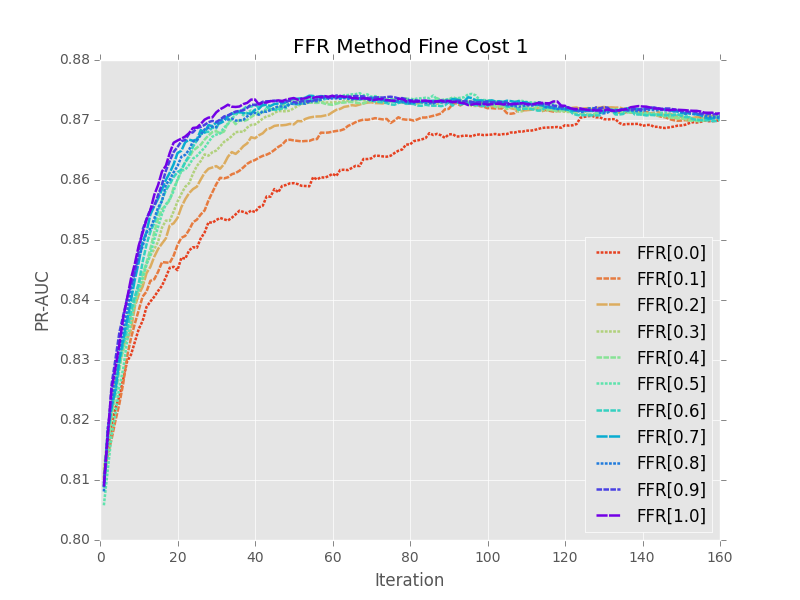
\includegraphics[ width=\paperwidth]{FFR_PR_Cost1}}
\par \textit{Figure:7}   The round size is changed to 160 and a fine has a cost of 1.
The 0p5 round for instance, corresponds to 0.5 of the total budget being used on fine,
so 80 goes to fine and 80 goes to coarse. For the 0p0 round, none of the budget is
used for fine and it has the worst performance. After around 0p3 the gains in performance
are marginal. The performance increases with the green 1p0 curve outperforming the
rest. The results are an average of 10 folds.\\
\makebox[\textwidth]{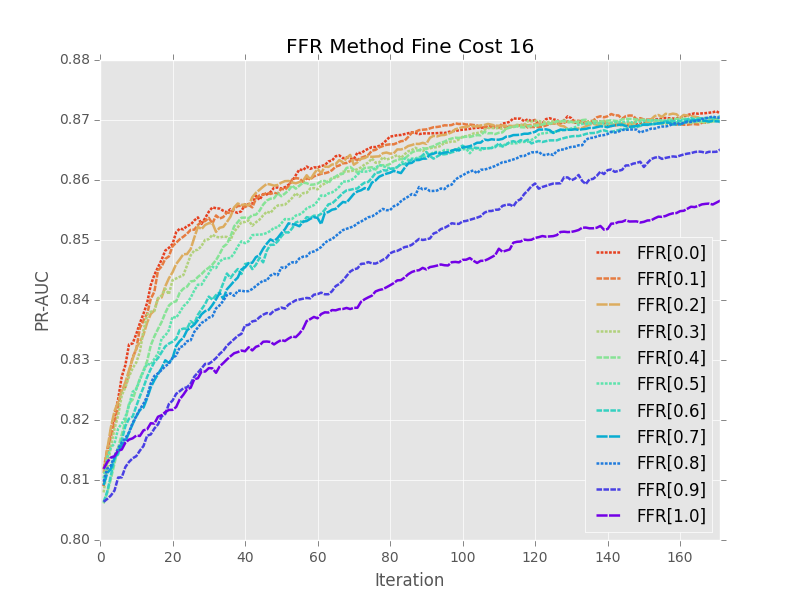
\includegraphics[width=\paperwidth]{FFR_PR_Cost16}}
\par \textit{Figure:8} The round size is again 160 and fine has a cost of 16.
The worst performing curve is again 0p0 with no fine instances, but the benefit of
fine instances is marginal. For the 0p5 case 5 instances are purchased for fine and
80 are purchased for coarse. For the 1p0 case 16 instances are purchase for fine and
144 instances are purchased for coarse.\\
\end{center}






\end{enumerate} % end sections






\end{document}  















